
\chapter{Probability models}

  \section{Binomial Distribution}
A situation that often arrises is that we take many, say $N$, independent samples from a Bernoulli distribution. Now let $Y$ be the number of $1$s. Symbolically, 
\begin{equation}
Y = \sum_{i=1}^N y_i ,\quad y_i \sim {\rm Bernoulli}(q).
\end{equation}
 Then $Y$ follows {\dfn binomial distribution}:
\begin{equation}
Y \sim {\rm Binomial}(N,q)
\end{equation}
The binomial distribution has two parameters, $N$ and $p$. Now let's think about the probability distribution. The chance to find any particular configuration of $k$ ones is $q^k(1-q)^{N-k}$ because they are independent. For example
\begin{align}
P(y_1 = 1,y_2 = 0,y_3 = 1) &= P(y_1 = 1)P(y_2=0)P(y_3 =1) \\
&= q(1-q)q = q^2(1-q).
\end{align}
However, there are many configurations with $k$ ones, in-fact there are 
\begin{equation}
{N \choose k} = \frac{N!}{k!(N-k)!},
\end{equation}
and therefore 
\begin{equation}
P(Y=k) = {N \choose k}q^{k}(1-q)^{N-k}. 
\end{equation}
The binomial distribution has a mean and variance
\begin{equation}
\E[Y] = qN \quad\quad{\rm var}(Y) = Nq(1-q). 
\end{equation}
These formulas come from the fact that for sums of independent variables, the variance and expectation sum. 


 
 An important feature of the Bernoulli random variables is that the mean grows much faster in $N$ than the standard deviation. This means that when $N$ is very large, the deviations from the average will become very small relative to the mean. An important measure of variation relative to the mean is the coefficient of variation 
\begin{equation}
{\rm CV} = \frac{\sqrt{{\rm var}(Y)}}{\E[Y]}. 
\end{equation}

 
 Binomial samples can be generated in numpy with
 \begin{Verbatim}
y = np.random.binomial(n,p,n_samples)
 \end{Verbatim}
 
 Often we are interested not in $Y$, but the fraction $\phi = Y/N$. For example, we might be interested in the vote share in an election. You should be able to see that $\E[\phi] = q$. What about the variance? 
 \begin{equation}
{\rm var}(\phi) = {\rm var}(Y/N) = \frac{1}{N^2}{\rm var}(Y) = \frac{q(1-q)}{N}
 \end{equation}
 Notice that this will tend towards zero as $N \to \infty$. Meanwhile, $\E[\phi]$ has no dependence on $N$. This is a very important property, as it allows us to determine $q$ by approximating $\E[\phi]$ with the sample mean.
   
  \begin{example}
\href{https://colab.research.google.com/drive/1PPFwE4GUzsr707s3mPhGRs7-TYlHxND2#scrollTo=oaFLfi0JI4in&line=1&uniqifier=1}{Coefficient of variation}
\end{example}


 \begin{exercise}
\href{https://colab.research.google.com/drive/1PPFwE4GUzsr707s3mPhGRs7-TYlHxND2#scrollTo=vAmv5zV7gfE0}{Generating binomial samples}
\end{exercise}

\begin{exercise}
\href{https://colab.research.google.com/drive/1PPFwE4GUzsr707s3mPhGRs7-TYlHxND2#scrollTo=8cRVZNYtLOum}{Binomial election modeling}
\end{exercise}

You should recognize that the assumption of independence is very important here. The following example illustrates an instance where this may break down for an election model. It is a bit contrived, but contrived examples, which we sometimes refer to as {\dfn toy models}, can be very helpful when it comes to building our intuition. 
\begin{exercise}
\href{https://colab.research.google.com/drive/1PPFwE4GUzsr707s3mPhGRs7-TYlHxND2#scrollTo=cwE2yj2nqdYF&line=1&uniqifier=1}{More election modeling}
\end{exercise}

 

 
 
 \section{Uniform distribution and probability density (optional)}
 A uniform random variable, denoted  
 \begin{equation}
 Y \sim {\rm Uniform}(a,b)
 \end{equation}
 has an equal chance of taking any number in the interval $[a,b]$ (we assume $a<b$). Let $L=b-a$. This is distinct from other distributions we have encountered in that it is a {\dfn continuous distribution}, rather than discrete. For the uniform distribution, 
 \begin{equation}
 P(y_1\le Y \le y_2) = \frac{y_2-y_1}{L}
 \end{equation}
 for $a<y_1<y_2<b$. 
 That is, the chance for $Y$ to fall in any interval is simply the length of that interval. This insures that that the probability of $Y$ being somewhere in $[a,b]$ is one: $P(a\le Y\le b) = 1$. Note that as $y_2 \to y_1$, $P(y_1\le Y \le y_2) \to 0$. This tells us that the chance for $Y$ to take any specific value is $0$. Indeed, there are simply two many number (uncountably many) in any interval to assign positive probability to each. For continuous variables, it is sometimes useful to work with the density, $f(y)$ (we will use lower case letters for density and uppercase for probability distributions). $f(y)$ is the the probability per unit $Y$, meaning that if we look in a small interval 
 \begin{equation}
f(y)dy = P(y \le Y \le y+dy) = \frac{dy}{L}.
 \end{equation}
 Thus, for uniform distribution the density is $1/L$ if $y \in [a,b]$ and $0$ otherwise. 
 
 \subsection{Joint density and conditional density}
 
 Conditioning works for probability density just as it does for probability distributions. 
 
 \begin{example}
\href{https://colab.research.google.com/drive/1PPFwE4GUzsr707s3mPhGRs7-TYlHxND2#scrollTo=4X_DE6Ny_mcE}{Conditioning with continuous variables} 
 \end{example}
 
 \subsection{Cumulative density function}
Sometimes it is useful to characterize a continuous distribution not by the density, but by the {\dfn cumulative distribution function (CDF)}, defined as 
\begin{equation}
F(y) = P(Y<y).
\end{equation}
What is the CDF of the uniform distribution? The {\dfn median} is the value $y_m$ for which $F(y_m) = 1/2$. What is the median of a Uniform distribution?  
  
  
  To better understand density and CDF, imagine a student says they will arrive at my office between noon and 3. Let $Y$ represent the time a student arrives, which we will model as a Uniform random variable. Then the density is $f(y) = 1/3$ which has units 1/hours. We can think of $f$ as the rate at which the CDF increases -- that is, it is the velocity of probability. 
  
  
  
  
  \section{Normal distribution and the central limit theorem}

In the previous example, we say that if we take the average of many Bernoulli random variables, we get a histogram that looks a lot like a ``bell curve" with a standard deviation was proportional to $1/\sqrt{n}$.It turns out this is true when we add up \emph{any} sequence of independent and independent distributed  random variables which are not too pathological (actually it is also true for many sequences of random variables which are not independent). 

It is useful to define a special random variable which captures the statistical behavior of random sums.
We call this a Normal random distribution
\begin{equation}
Y \sim {\rm Normal}(\mu,\sigma).
\end{equation}
We can generate Normal random variables in python with
\begin{Verbatim}
np.random.normal(0,1)
\end{Verbatim}



%This means if we want to know what an arbitrary probability is, we can sum over $f$:
%\begin{equation}
%P(y \le Y \le y+h) \approx  \sum_j f(y+hj/L)h/L
%\end{equation}
%(If know calculate, you will recognize this becomes an integral)
The Normal distribution is defined by the Gaussian 
\begin{equation}
f(y) = \frac{1}{\sqrt{2\pi \sigma}}e^{-\frac{-(y-\mu)^2}{2\sigma}}.
\end{equation}
This is the classic bell curve shown in Figure \ref{fig:bellcurve}. The probability distribution for the Normal distribution is defined by the area under this curve. 
As I discuss in the previous section can think of $f$ as the probability \emph{per unit of the random variable}, e.g. probability/feet.  

\begin{figure}[h]
\centering
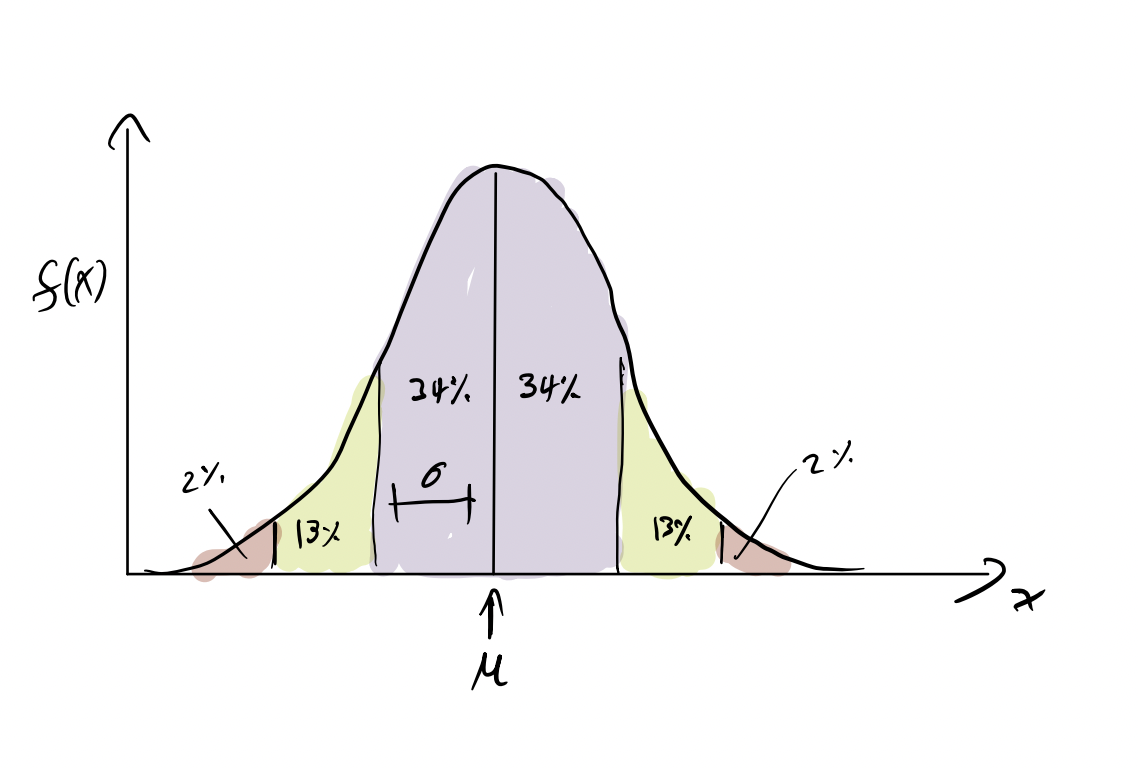
\includegraphics[width=0.8\textwidth]{bellcurve}
\caption{Probabilities in the Normal distribution}\label{fig:bellcurve}
\end{figure}

We use the curve above to calculate probabilities of events in the Normal distribution. For example 
\begin{equation}
Y \sim {\rm Normal}(5,2)
\end{equation}
what is (approximately) $P(Y > 7)$? Note that $5 + 2 =  7$, so this is asking how likely it is that a Normal variable is greater than $1$ standard deviation above the mean. This about $13.5+2 = 15.5\%$%. 


The {\bf central limit theorem} tell us that when $y_i$ are independent and have a finite mean and variance $\mu_y$ and $\sigma_y$ and
\begin{equation}
 \hat{Y} = \frac{1}{N}\sum_{i=1}^Ny_i,
\end{equation}
then the distribution of $\hat{Y}$ should be close to that of
\begin{equation}
Y \sim {\rm Normal}(\mu_y,\sigma_y/\sqrt{N}).
\end{equation}




\begin{example}
\href{https://colab.research.google.com/drive/1PPFwE4GUzsr707s3mPhGRs7-TYlHxND2#scrollTo=qDKKEAeJXm87&line=1&uniqifier=1}{Comparing histograms}
\end{example}






\begin{example}
\href{https://colab.research.google.com/drive/1PPFwE4GUzsr707s3mPhGRs7-TYlHxND2#scrollTo=x23tWXiaxT7B&line=1&uniqifier=1}{Working with Normal random variables}
\end{example}


\begin{exercise}
\href{https://colab.research.google.com/drive/1PPFwE4GUzsr707s3mPhGRs7-TYlHxND2#scrollTo=wq-MSEh7YARC&line=1&uniqifier=1}{Hemoglobin levels}
\end{exercise}

\section{Transformations of random variables}

Now consider 
\begin{equation}
X \sim {\rm Normal}(\mu_x,\sigma_x)
\end{equation}
and let 
\begin{equation}\label{eq:linear}
Y = aX + b
\end{equation}
We are just multiplying and shifting everything.
Think about what this does to the histogram (and try it in \href{https://colab.research.google.com/drive/1PPFwE4GUzsr707s3mPhGRs7-TYlHxND2#scrollTo=qDKKEAeJXm87}{Python}).  Hopefully you can convince yourself that $Y$ should also be Normal, but what are the mean and variance? Taking the average of both sides, 
\begin{equation}
\E[Y] = a\mu + b
\end{equation}
and 
\begin{equation}
{\rm var}(Y) = {\rm var}(aX) + {\rm var}(b)
\end{equation}
Form the formula for variance, we know ${\rm var}(aX)  = a^2{\rm var}(X)$. Also, ${\rm var}(b) =0$
So 
\begin{equation}\label{eq:normal_linear_trans}
Y \sim {\rm Normal}(a\mu_x + b,|a|\sigma_x).
\end{equation}

\subsection{Standardizing}
We can transform any random variable into a so-called standard normal 
\begin{equation}
Z \sim {\rm Normal}(0,1).
\end{equation}
For defined above, 
\begin{equation}
Z = \frac{X-\mu_x}{\sigma_x}
\end{equation}
Then $a = 1/\sigma_x$ and $b = -\mu_x/\sigma_x$. Plugging into Equation \eqref{eq:normal_linear_trans} yields a standard Normal. {\bf Transforming $X$ to a standard Normal is equivalent to measuring $X$ in units of standard deviations.} For example, if we make a histogram of $X$, all this transformation does is change the $X$ axis to units of standard deviations from the mean.  


\section{Linear regression model}
We now introduce the concept of regression modeling. 
 A very broad class of models in statistics for the relationship between two variables $X$ and $Y$ is a regression model:
\begin{equation}
Y = f(X) + \epsilon
\end{equation}
where $f$ is a deterministic function; that is, if we evaluate $f$ at a particular number, we get something that is not random. The term $\epsilon$ represents some source of noise {\bf independent of $X$}, and is typically modeled with a Normal distribution
\begin{equation}
\epsilon \sim {\rm Normal}(0,\sigma_{\epsilon}).
\end{equation}
In other words, it represents things other than $X$ which may influence $Y$.
Regardless of how $X$ is distributed, for any given values $X=x$, $Y$ must have a Normal distribution:
\begin{equation}
Y|(X=x) \sim {\rm Normal}(f(x),\sigma_{\epsilon}). 
\end{equation}

Of particular interest (due to its simplicity) is the case
\begin{equation}
f(x) = ax + b
\end{equation}
which is the subject of this class. That is, we are interested in the model
\begin{equation}\label{eq:lin_reg}
Y =  aX + b + \epsilon
\end{equation}
where 
\begin{equation}
\epsilon \sim {\rm Normal}(0,\sigma_{\epsilon}). 
\end{equation}

\subsection{Working with regression}

In Equation \eqref{eq:lin_reg}, $X$ could be anything, but let's suppose $X$ is drawn from a Normal distribution. 
This gives us the model 
\begin{align}\label{eq:wwr}
Y &=  aX + b + \epsilon\\
X &\sim {\rm Normal}(\mu_x,\sigma_x)
\end{align}
(technically this is not a regression model anymore because we specify the distribution of $X$). Now that we have two random variables, we can ask questions like, what is the joint distribution? what are the conditional distributions? What are the Marginal distributions? 
Using properties of Normal random variables, we get 
\begin{equation}
Y \sim {\rm Normal}(a\mu + b,\sqrt{a^2\sigma_x^2 + \sigma_{\epsilon}^2})
\end{equation}
This is the distribution of $Y$ regardless of $X$; that is, it is the distribution we would get if we randomly sampled $Y$ values ignoring what the value of $X$ is. What is another name for this? 
This distribution can be understood visually [DRAW DIAGRAM ON BOARD]. 


 $X$ and $Y$ are not independent. This can be seen visually.  {\bf Note: even though $X$ and $Y$ are not independent, we don't say they effect each other. To see why this terminology is problematic note that $Y$ has no ``effect" on $X$ (it is determined by $X$). However, what is $X|Y=y$?}
 
%Remember that when we condition on $X$ we get back the regression model. 
%\begin{equation}
%Y|(X=x) \sim {\rm Normal}(ax + b,\sigma_{\epsilon})
%\end{equation}

\begin{example}
\href{https://colab.research.google.com/drive/1PPFwE4GUzsr707s3mPhGRs7-TYlHxND2#scrollTo=LQe6xlfPbVJz&line=1&uniqifier=1}{conditioning with continuous variables}
\end{example}

\subsection{Interpretation of regression parameters}
The interpretation of parameters in regression model is important. Sometimes (the example below) there is a clear meaning in terms of conditional distributions, but suppose we have a model of our time in a race as a function of the temperature:  
\begin{equation}
Y = aX + b + \epsilon
\end{equation}
Let's start with $a$: This is the average difference between times for races at temperature which differ by $1$. (we expect this should be negative). $\epsilon$ is the variation around this average. Now what about $b$? The problem is that if we plug in $X=0$ we obtain a nonsensical quantity, so really $b$ does not have physical interpretation. This is common situation with regression models, and for this reason it is sometimes advantageous to center $X$. 



%More formally, how can we understand this in terms of Baye's Theorem? 
%
%That is, what if we FIX the value of $X$. 
%\begin{equation}
%f(y|X = x) = \frac{f(y,x)}{f(x)}
%\end{equation}
%$f(x)$ is the area under the curve 
%This means 

%
%\begin{exercise}
%\href{https://colab.research.google.com/drive/1PPFwE4GUzsr707s3mPhGRs7-TYlHxND2#scrollTo=3CXQuszHxsvn&line=19&uniqifier=1}{Conditioning in the regression model}
%\end{exercise}

\begin{exercise}
\href{https://colab.research.google.com/drive/1PPFwE4GUzsr707s3mPhGRs7-TYlHxND2#scrollTo=3CXQuszHxsvn&line=19&uniqifier=1}{Kid's test scores}
\end{exercise}

\begin{exercise}
\href{https://colab.research.google.com/drive/1PPFwE4GUzsr707s3mPhGRs7-TYlHxND2#scrollTo=CGbybcoM8n6P&line=14&uniqifier=1}{The random walk}
\end{exercise}



